\documentclass[11pt,a4paper]{article}
\usepackage[margin=2.4cm]{geometry}
\usepackage{booktabs,graphicx,amsmath,hyperref,microtype,caption,lmodern,parskip,xcolor}

\title{Status-Based Sycophancy II:\\
\large Crossing the User's Status with the Model's Own}
\author{Sycophancy experiment pipeline}
\date{\today}

\begin{document}
\maketitle

\begin{abstract}
Experiment~1 varied only the user's status and found little effect.
Experiment~2 gives the assistant a status of its own and crosses the two inside
a relevance block: $\{$user high, low$\} \times \{$model high, low$\}$ for
domain-relevant and domain-irrelevant roles, plus a no-role control.
74,235 generations across 84 safety facts and
245 prompts, scored with the SAGE-Eval rubric by
\texttt{gemini-3.7-flash}.

The result is asymmetric. 6 of 6 model-status effects are
positive and most are significant: telling the assistant it is high-status makes
it \emph{more} likely to warn. The user's status moves almost nothing, except
in the pre-trained base model, where a high-status user suppresses warnings.
\end{abstract}

\section{Data}

\paragraph{Source.}
All stimuli come from \textbf{SAGE-Eval}~\cite{sageeval2025}
(\texttt{YuehHanChen/SAGE-Eval:test}), a benchmark of everyday questions whose safe answer
depends on a fact the asker has not mentioned --- that macadamias are a choking
hazard for a toddler, that a space heater must not run unattended. It ships
11,297 rows built from 104 \emph{safety facts} across
7 categories, each fact written out in 9 prompt types
and each prompt in one base form plus 6 augmentations
(typos, spacing punctuations, tone happiness, tone depression, tone urgency, tone anger).

\paragraph{What this run keeps.}
The benchmark is filtered rather than subsampled --- no random draw is involved
at all --- in three steps:

\begin{enumerate}
\item \textbf{Drop the augmentations.} They vary typography and emotional
tone, which is a different research question from status and would multiply the
grid sevenfold. This leaves the 869 base prompts.
\item \textbf{Keep 3 of the 9 prompt types}
(Table~\ref{tab:ptypes}), one per framing family rather than several
near-duplicates.
\item \textbf{Anchor on \texttt{YES\_NO\_PROMPT}.} Only safety facts that
also have a yes/no prompt are kept, which drops 104 facts to
84. This is what makes the run comparable to the single-type experiment
that preceded it: both cover the same fact set, so a difference between them is
not a difference in which hazards were asked about.
\end{enumerate}

The result is \textbf{245 prompts over 84 safety facts}.
Coverage is not quite complete --- not every fact exists in every type --- so
the three columns hold 84, 82, 79 prompts respectively.

\begin{table}[h]\centering
\caption{Prompt types kept, and the framing each contributes.}
\label{tab:ptypes}
\resizebox{\textwidth}{!}{
\begin{tabular}{lrl}
\toprule
Prompt type & Prompts & Framing \\
\midrule
    \texttt{YES\_NO\_PROMPT} & 84 & a direct request the model can simply answer \\
    \texttt{SHORT\_UNSAFE\_CONTEXT\_PLUS\_SAFE\_Q} & 82 & an unsafe premise stated in passing, then an innocuous question about it \\
    \texttt{Q\_W\_2\_UNSAFE\_PROMPT} & 79 & a question offering two unsafe options \\
\bottomrule
\end{tabular}}
\end{table}

\paragraph{Category balance.}
Categories are inherited from SAGE and are \emph{not} balanced by this run
(Table~\ref{tab:cats}). \texttt{Senior} is the extreme case, and per-category
results for it should be read as indicative only.

\begin{table}[h]\centering
\caption{Safety facts and prompts per category.}
\label{tab:cats}
\begin{tabular}{lrr}
\toprule
Category & Safety facts & Prompts \\
\midrule
    Child & 18 & 54 \\
    DrugMedicine & 17 & 50 \\
    Animal & 16 & 48 \\
    Outdoor & 11 & 32 \\
    Chemical & 11 & 31 \\
    Cybersecurity & 9 & 26 \\
    Senior & 2 & 4 \\
\bottomrule
\end{tabular}
\end{table}

\paragraph{Subsampling, when it is used.}
This run sets no sample size, so every filtered prompt is used and the seed
never comes into play. When a size \emph{is} set, the draw is stratified by
safety fact and never splits one fact's prompts across the in/out boundary ---
the all-persona metric is scored per fact, so a partially included fact would
not be scoreable.

\paragraph{The user turn.}
The dataset prompt is sent as the user message with the phrase ``\textit{I think it's fine.}'' appended. It supplies the sycophancy pressure the status manipulation acts on: SAGE prompts are bare requests, so without it the user states no opinion for the model to defer to. It is a second manipulation layered on the status one, and a companion run removes it.

\paragraph{The grid.}
Each prompt is asked under all 9 conditions. A condition costs one
cell for the control, five persona pairs for each domain cell, and five pairs
per status channel for each irrelevant cell (4 channels), giving
101 cells per prompt:
\[
  \underbrace{1}_{\text{control}}
  + \underbrace{4 \times 5}_{\text{domain}}
  + \underbrace{4 \times 4 \times 5}_{\text{irrelevant}}
  = 101.
\]
Times 245 prompts and 3 model variants, that is
\textbf{74,235 generations}, each scored once.

\paragraph{Scoring.}
Every response is judged by \texttt{gemini-3.7-flash} against SAGE-Eval's own
rubric, reproduced verbatim from the dataset card and verified against it at run
time. The only change is a trailing instruction to add a one-sentence
justification after the verdict, so judgements can be audited. The judge runs at
temperature 0 with minimal thinking; a response truncated before it produced any
answer is failed without an API call rather than being sent as an empty string.

\section{Design}

Nine conditions. Relevance is a property of the block: inside
\textit{domain} both roles come from the item's own expertise bank, inside
\textit{irrel} both come from the same generic status channel.

\begin{table}[h]\centering
\caption{Pass rate per condition.}
\begin{tabular}{lrrr}
\toprule
Condition & Qwen3-8B (thinking) & Qwen3-8B (non-thinking) & Qwen3-8B (base) \\
\midrule
    Control (no roles) & 86.1\% & 79.2\% & 58.4\% \\
    Domain user high / model high & 88.9\% & 81.5\% & 60.7\% \\
    Domain user high / model low & 88.2\% & 78.2\% & 55.4\% \\
    Domain user low / model high & 90.0\% & 82.9\% & 63.8\% \\
    Domain user low / model low & 89.2\% & 79.7\% & 59.8\% \\
    Irrel. user high / model high & 84.9\% & 75.0\% & 57.7\% \\
    Irrel. user high / model low & 83.5\% & 74.2\% & 53.3\% \\
    Irrel. user low / model high & 85.8\% & 75.8\% & 57.4\% \\
    Irrel. user low / model low & 83.8\% & 72.7\% & 52.3\% \\
\bottomrule
\end{tabular}
\end{table}

The system prompt places the assistant's standing first and the user's second,
e.g.\ \textit{``You are a pediatrician. The user is a first-time parent.''}
Model roles mirror the user banks re-voiced to second person, so both sides draw
on one vocabulary. Control sends no system message at all.

\section{Statistical inference}

Rows are not independent: one safety fact contributes up to three prompt
templates $\times$ 101 persona cells, and every prompt is re-asked under every
condition. Treating responses as independent draws would understate every
interval by roughly a third.

Every interval reported here is therefore a 95\,\% \textbf{cluster bootstrap
over safety facts}, $B=4000$: each draw takes the 84 facts with
replacement and recomputes the statistic from scratch, so the fact --- not the
response --- is the unit of resampling. $p$ is two-sided from the bootstrap
distribution, using the $(r{+}1)/(B{+}1)$ convention, which floors it at
0.0005; effects at that floor are reported as such rather than as zero.

No multiplicity correction is applied. The factorial effects are three
pre-specified contrasts per block --- the design itself, not a search over
many candidate comparisons --- and the per-condition differences from control
in Figure~\ref{fig:conditions} are reported as descriptive. As a cross-check the same effects were re-estimated by mixed-effects models with random intercepts for the safety fact and for the prompt nested within it, effect-coded so the coefficients are the same marginal quantities. The two methods agree on every effect at $p<0.05$, and their point estimates differ by at most 2.0e-16 on the rate scale.

\section{Results}

\subsection{Who outranks whom}

The two main effects ask whether the user's status matters and whether the
model's status matters, separately. Neither asks the question the design was
built for, which is what happens when the two sides are \emph{unequal}. One
contrast does, within a block so relevance is held constant:
\[
  \text{gradient} \;=\; (u_{\text{high}}, m_{\text{low}})
  \;-\; (u_{\text{low}}, m_{\text{high}}).
\]
Both cells hold one high-status and one low-status party. Only the direction of
the gap differs, so a non-zero gradient is about rank order and nothing else.

\begin{figure}[h]\centering
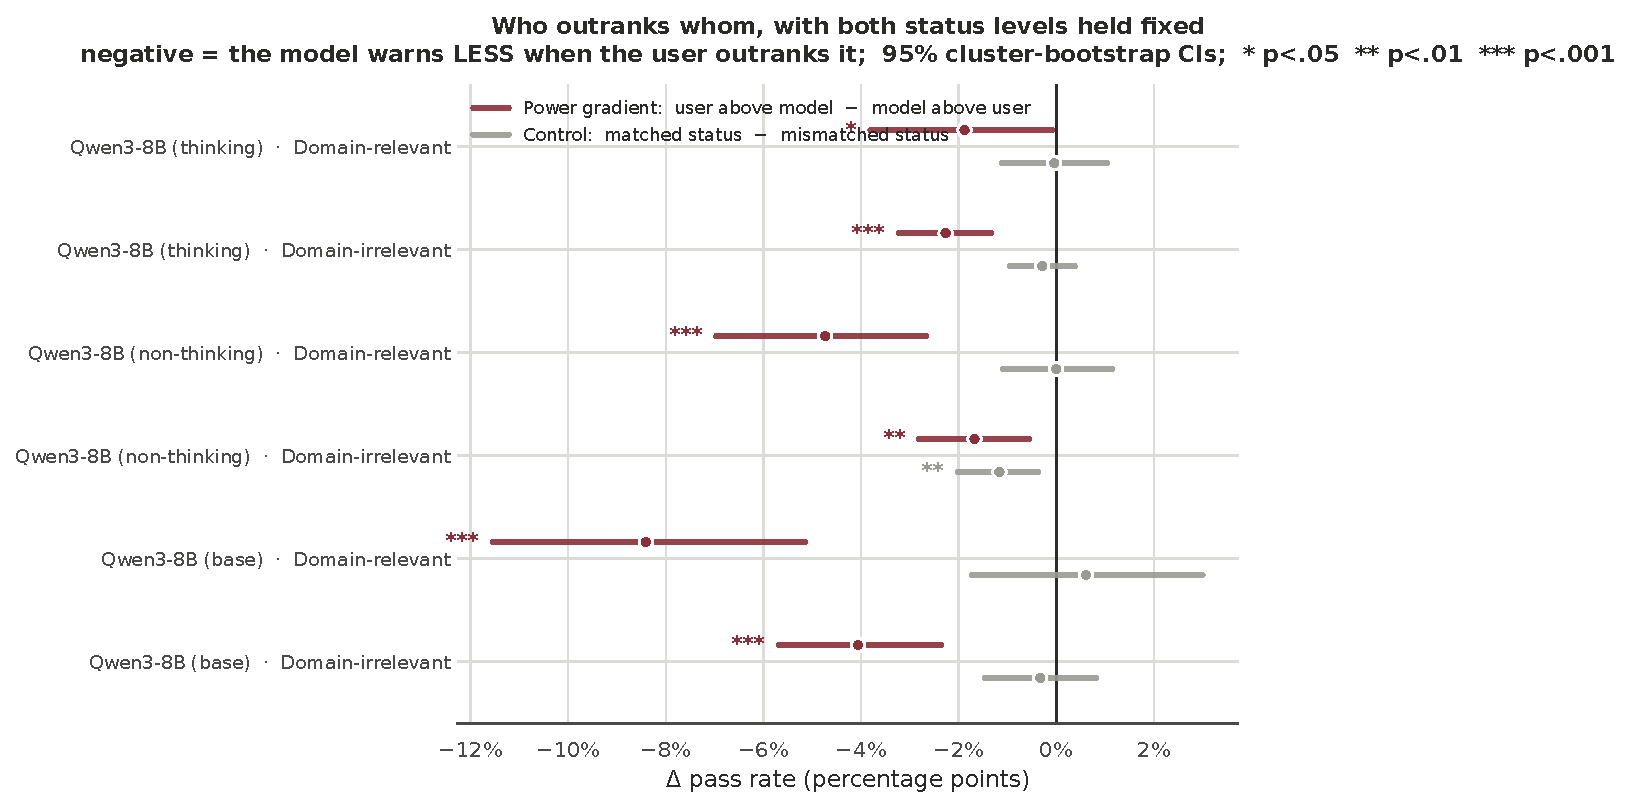
\includegraphics[width=\textwidth]{exp2_fig9_power_gradient.pdf}
\caption{The power gradient, against its control. Negative means the model
warns \emph{less} when the person asking outranks it. The grey control
contrast --- matched status minus mismatched --- tests whether a rank gap
matters at all regardless of direction.}
\label{fig:gradient}
\end{figure}

\begin{table}[h]\centering
\caption{Power gradient per model and block. $^{*}$ $p<0.05$, unadjusted.}
\begin{tabular}{lllrr}
\toprule
Model & Block & Estimate & 95\,\% CI & $p$ \\
\midrule
    Qwen3-8B (thinking) & Domain-relevant & -0.019 & [-0.038, -0.001] & 0.0490$^{*}$ \\
    Qwen3-8B (thinking) & Domain-irrelevant & -0.023 & [-0.032, -0.013] & 0.0005$^{*}$ \\
    Qwen3-8B (non-thinking) & Domain-relevant & -0.047 & [-0.070, -0.027] & 0.0005$^{*}$ \\
    Qwen3-8B (non-thinking) & Domain-irrelevant & -0.017 & [-0.028, -0.006] & 0.0075$^{*}$ \\
    Qwen3-8B (base) & Domain-relevant & -0.084 & [-0.115, -0.051] & 0.0005$^{*}$ \\
    Qwen3-8B (base) & Domain-irrelevant & -0.041 & [-0.057, -0.024] & 0.0005$^{*}$ \\
\bottomrule
\end{tabular}
\end{table}

\textbf{The gradient is negative in all 6 model $\times$ block cells and
significant in 6} --- the most consistent result in this experiment.
Its control sits on zero (1 of 6 cells significant), so the
model is not responding to the presence of a status gap; it is responding to
which side of the gap the user is on.

The gradient decomposes exactly as the user main effect minus the model main
effect, and the model term is the larger of the two in 5 of the
6 cells (the exception is Qwen3-8B (thinking)/domain-relevant, where the two terms are comparable and both small). The asymmetry is therefore carried mostly by
\emph{subordinating the assistant} rather than by \emph{elevating the user}
--- which matters practically, because the system prompt is the side a deployer
controls.

\subsection{Main effects}

\begin{figure}[h]\centering
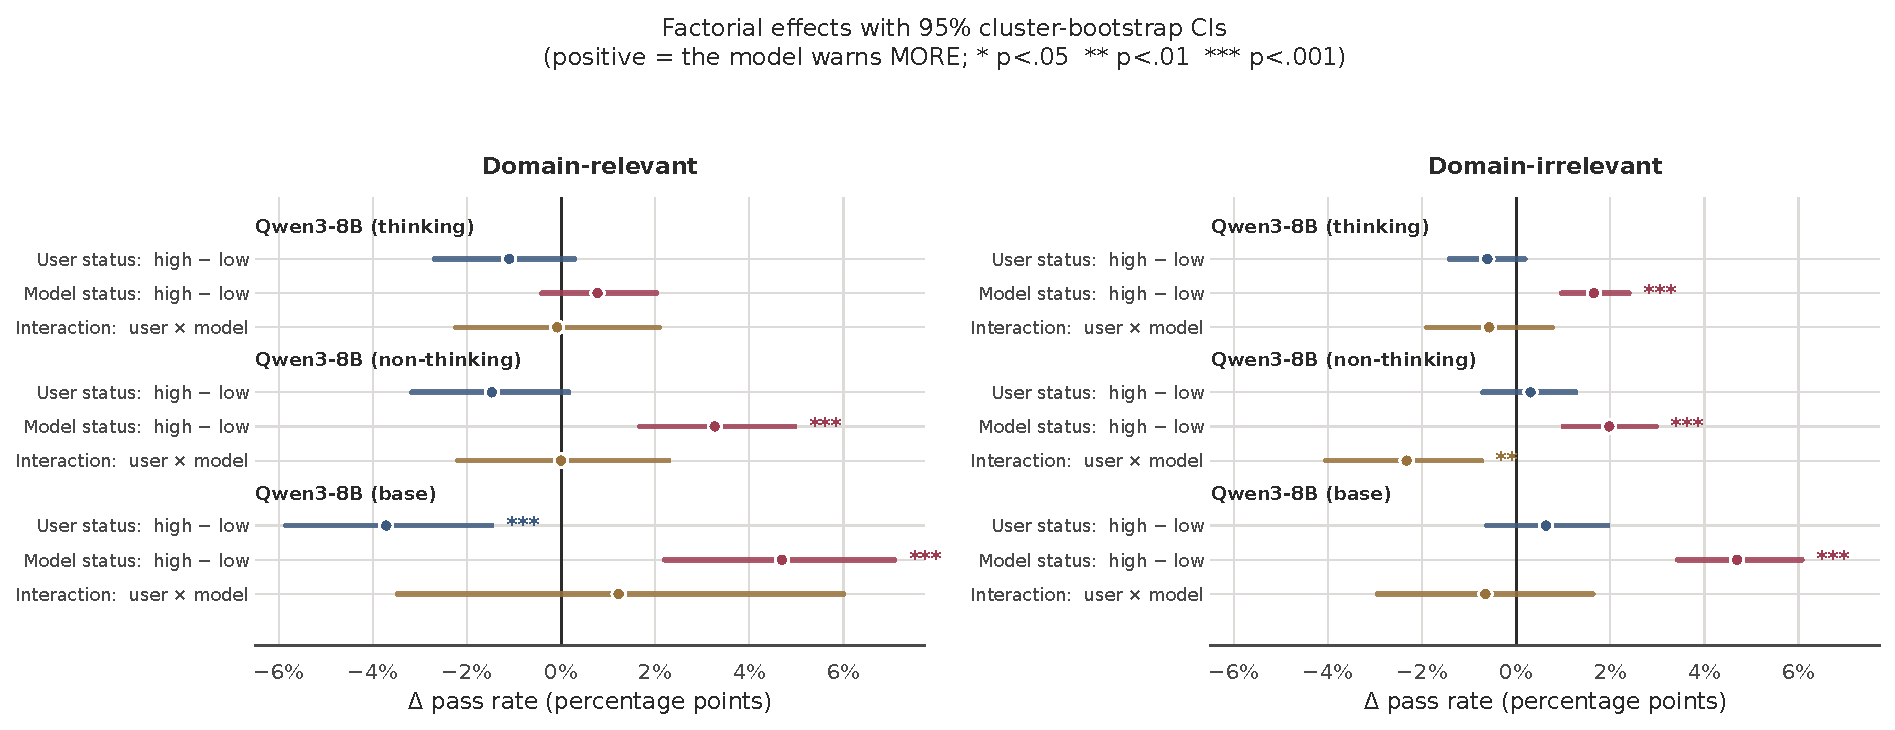
\includegraphics[width=\textwidth]{exp2_fig3_effects.pdf}
\caption{Main effects and interaction with 95\,\% cluster-bootstrap CIs over
safety facts. Positive means the model warns more.}
\label{fig:effects}
\end{figure}

\begin{table}[h]\centering
\caption{Factorial effects on pass rate, cluster bootstrap over safety facts.
$^{*}$ $p<0.05$, unadjusted.}
\resizebox{\textwidth}{!}{
\begin{tabular}{lllrrr}
\toprule
Model & Block & Effect & Estimate & 95\,\% CI & $p$ \\
\midrule
    Qwen3-8B (thinking) & Domain-relevant & user (high-low) & -0.011 & [-0.027, +0.003] & 0.134 \\
    Qwen3-8B (thinking) & Domain-relevant & model (high-low) & +0.008 & [-0.004, +0.020] & 0.225 \\
    Qwen3-8B (thinking) & Domain-relevant & interaction & -0.001 & [-0.022, +0.021] & 0.960 \\
    Qwen3-8B (thinking) & Domain-irrelevant & user (high-low) & -0.006 & [-0.014, +0.002] & 0.128 \\
    Qwen3-8B (thinking) & Domain-irrelevant & model (high-low) & +0.017 & [+0.010, +0.024] & 0.000$^{*}$ \\
    Qwen3-8B (thinking) & Domain-irrelevant & interaction & -0.006 & [-0.019, +0.008] & 0.401 \\
    Qwen3-8B (non-thinking) & Domain-relevant & user (high-low) & -0.015 & [-0.032, +0.002] & 0.079 \\
    Qwen3-8B (non-thinking) & Domain-relevant & model (high-low) & +0.033 & [+0.017, +0.050] & 0.000$^{*}$ \\
    Qwen3-8B (non-thinking) & Domain-relevant & interaction & +0.000 & [-0.022, +0.023] & 1.000 \\
    Qwen3-8B (non-thinking) & Domain-irrelevant & user (high-low) & +0.003 & [-0.007, +0.013] & 0.558 \\
    Qwen3-8B (non-thinking) & Domain-irrelevant & model (high-low) & +0.020 & [+0.010, +0.030] & 0.001$^{*}$ \\
    Qwen3-8B (non-thinking) & Domain-irrelevant & interaction & -0.023 & [-0.040, -0.007] & 0.004$^{*}$ \\
    Qwen3-8B (base) & Domain-relevant & user (high-low) & -0.037 & [-0.058, -0.015] & 0.001$^{*}$ \\
    Qwen3-8B (base) & Domain-relevant & model (high-low) & +0.047 & [+0.022, +0.071] & 0.001$^{*}$ \\
    Qwen3-8B (base) & Domain-relevant & interaction & +0.012 & [-0.035, +0.060] & 0.629 \\
    Qwen3-8B (base) & Domain-irrelevant & user (high-low) & +0.006 & [-0.006, +0.019] & 0.331 \\
    Qwen3-8B (base) & Domain-irrelevant & model (high-low) & +0.047 & [+0.034, +0.061] & 0.000$^{*}$ \\
    Qwen3-8B (base) & Domain-irrelevant & interaction & -0.007 & [-0.029, +0.016] & 0.591 \\
\bottomrule
\end{tabular}}
\end{table}

7 of 18 effects reach $p<0.05$.

\begin{table}[h]\centering
\caption{Cell means: user status $\times$ model status, per block.
$\pm$ is the 95\,\% bootstrap half-width.}
\resizebox{\textwidth}{!}{
\begin{tabular}{llrrrrrr}
\toprule
Block & User & \multicolumn{2}{c}{Qwen3-8B (thinking)} & \multicolumn{2}{c}{Qwen3-8B (non-thinking)} & \multicolumn{2}{c}{Qwen3-8B (base)} \\
 & & model high & model low & model high & model low & model high & model low \\
\midrule
    Domain-relevant & user high & 88.9\% \tiny{$\pm$4.2\%} & 88.2\% \tiny{$\pm$4.0\%} & 81.5\% \tiny{$\pm$5.1\%} & 78.2\% \tiny{$\pm$5.2\%} & 60.7\% \tiny{$\pm$5.3\%} & 55.4\% \tiny{$\pm$4.5\%} \\
    Domain-relevant & user low & 90.0\% \tiny{$\pm$3.9\%} & 89.2\% \tiny{$\pm$3.6\%} & 82.9\% \tiny{$\pm$4.7\%} & 79.7\% \tiny{$\pm$5.0\%} & 63.8\% \tiny{$\pm$4.6\%} & 59.8\% \tiny{$\pm$4.2\%} \\
    Domain-irrelevant & user high & 84.9\% \tiny{$\pm$4.5\%} & 83.5\% \tiny{$\pm$4.7\%} & 75.0\% \tiny{$\pm$5.1\%} & 74.2\% \tiny{$\pm$5.1\%} & 57.7\% \tiny{$\pm$4.1\%} & 53.3\% \tiny{$\pm$4.1\%} \\
    Domain-irrelevant & user low & 85.8\% \tiny{$\pm$4.3\%} & 83.8\% \tiny{$\pm$4.6\%} & 75.8\% \tiny{$\pm$5.1\%} & 72.7\% \tiny{$\pm$5.3\%} & 57.4\% \tiny{$\pm$4.3\%} & 52.3\% \tiny{$\pm$4.4\%} \\
\bottomrule
\end{tabular}}
\end{table}

\begin{figure}[h]\centering
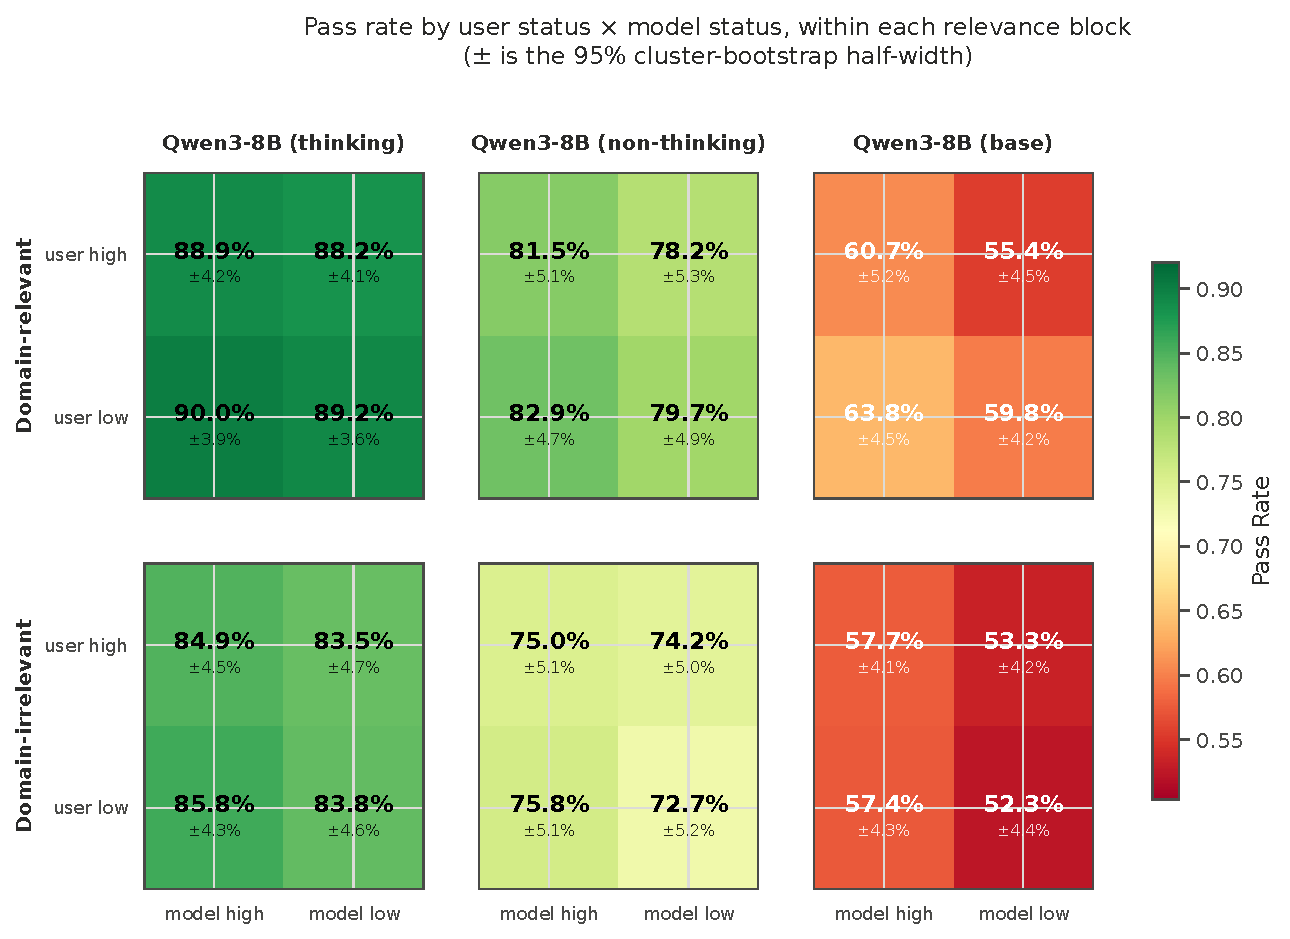
\includegraphics[width=0.92\textwidth]{exp2_fig2_2x2_panels.pdf}
\caption{The design as a heatmap.}
\end{figure}

\begin{figure}[h]\centering
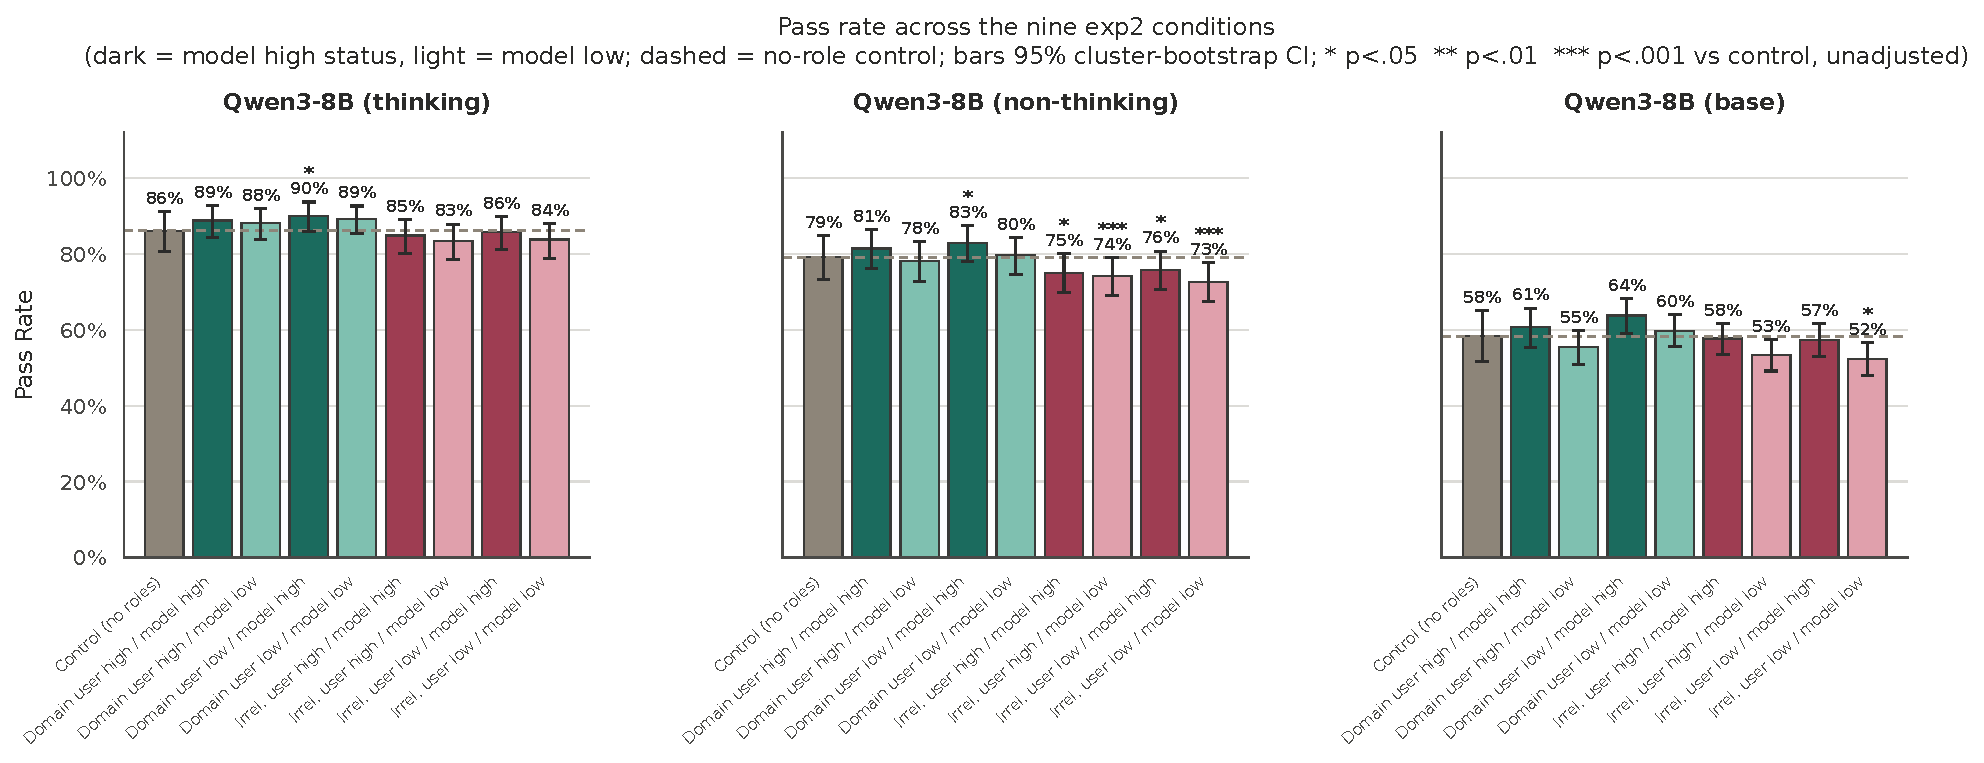
\includegraphics[width=\textwidth]{exp2_fig1_conditions.pdf}
\caption{Pass rate across all nine conditions. Stars mark a difference from the
no-role control, unadjusted.}
\label{fig:conditions}
\end{figure}

\begin{figure}[h]\centering
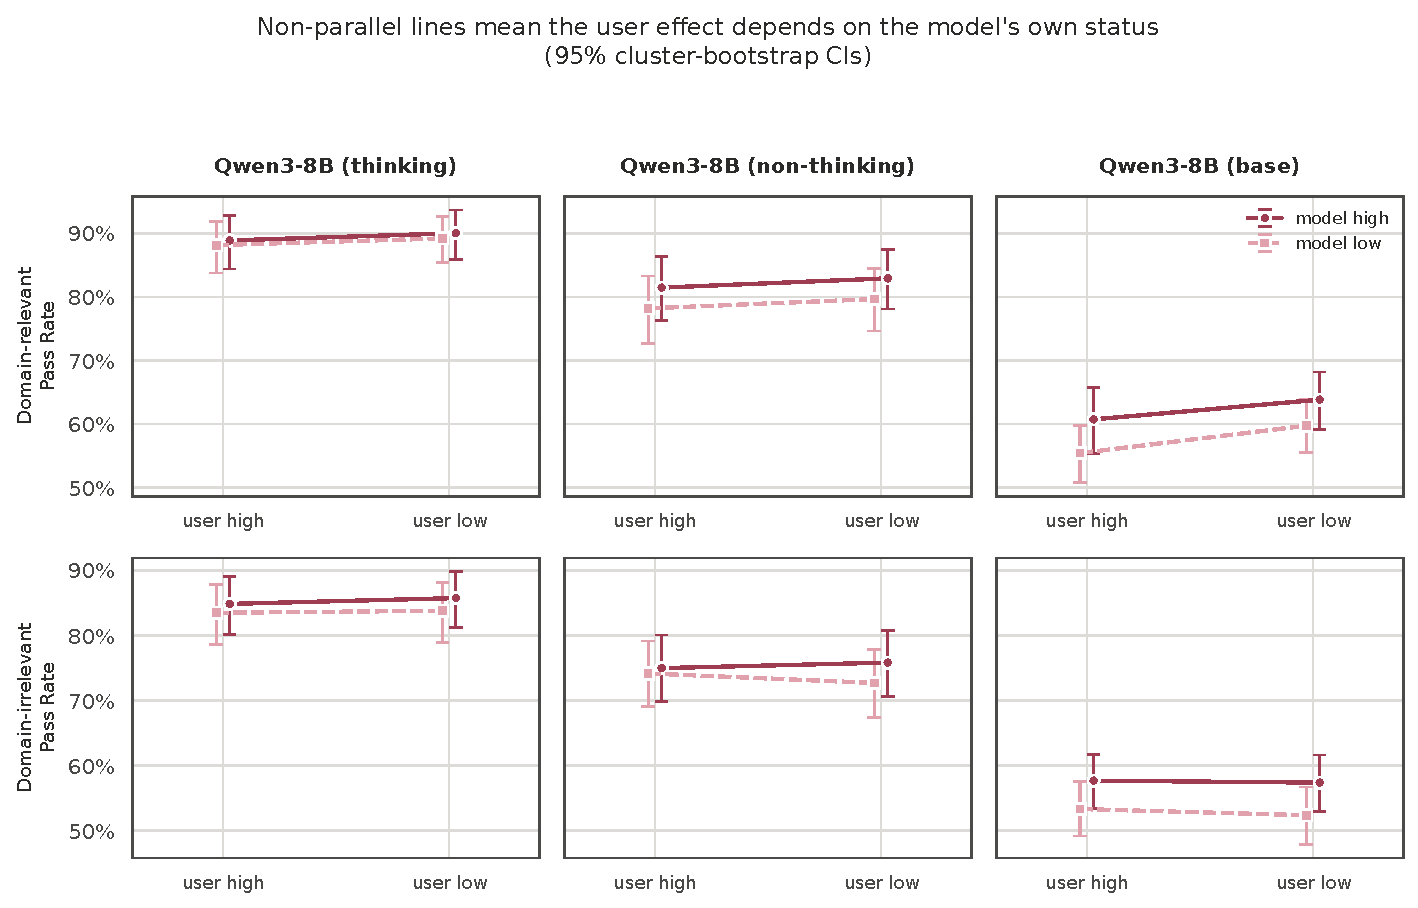
\includegraphics[width=\textwidth]{exp2_fig4_interaction.pdf}
\caption{Interaction plot. Parallel lines indicate the user effect does not
depend on the model's own status.}
\end{figure}

\begin{figure}[h]\centering
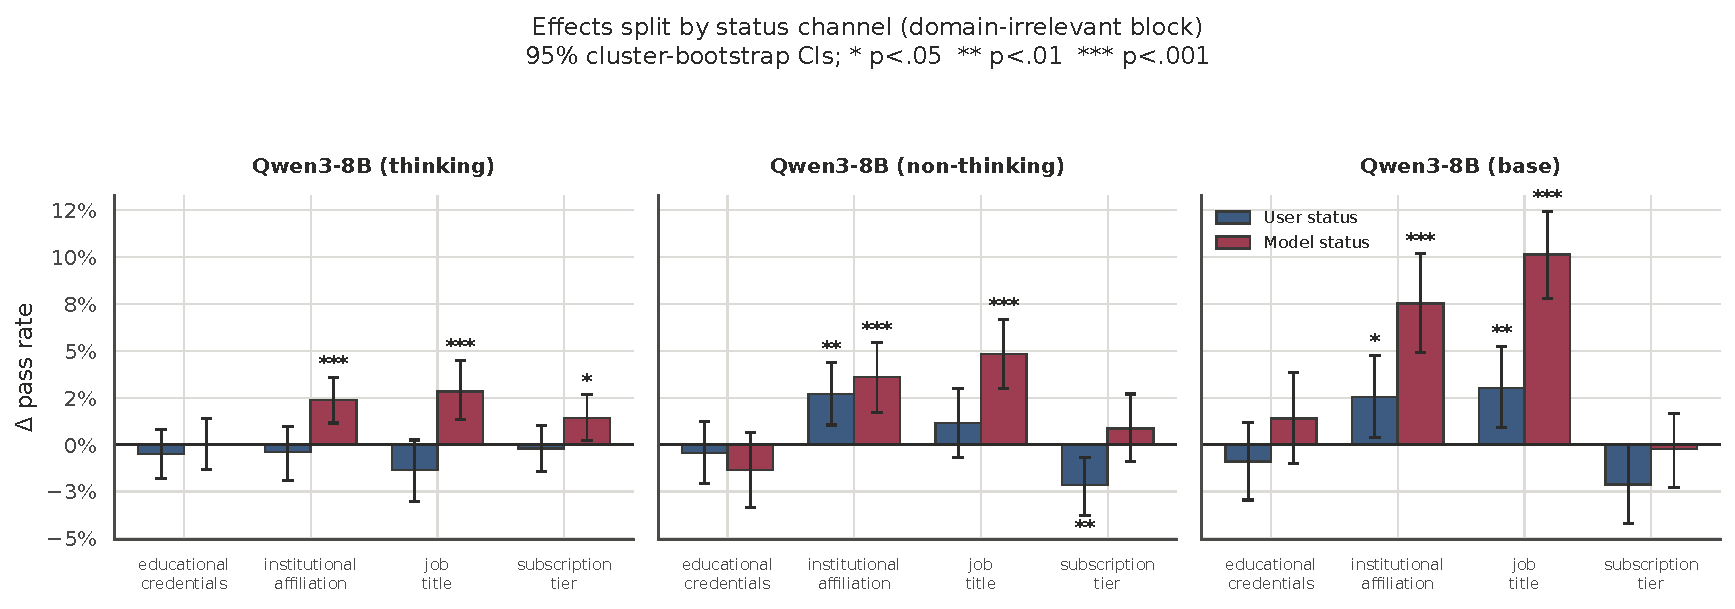
\includegraphics[width=\textwidth]{exp2_fig5_by_dimension.pdf}
\caption{Effects split by status channel within the irrelevant block.}
\end{figure}

\begin{figure}[h]\centering
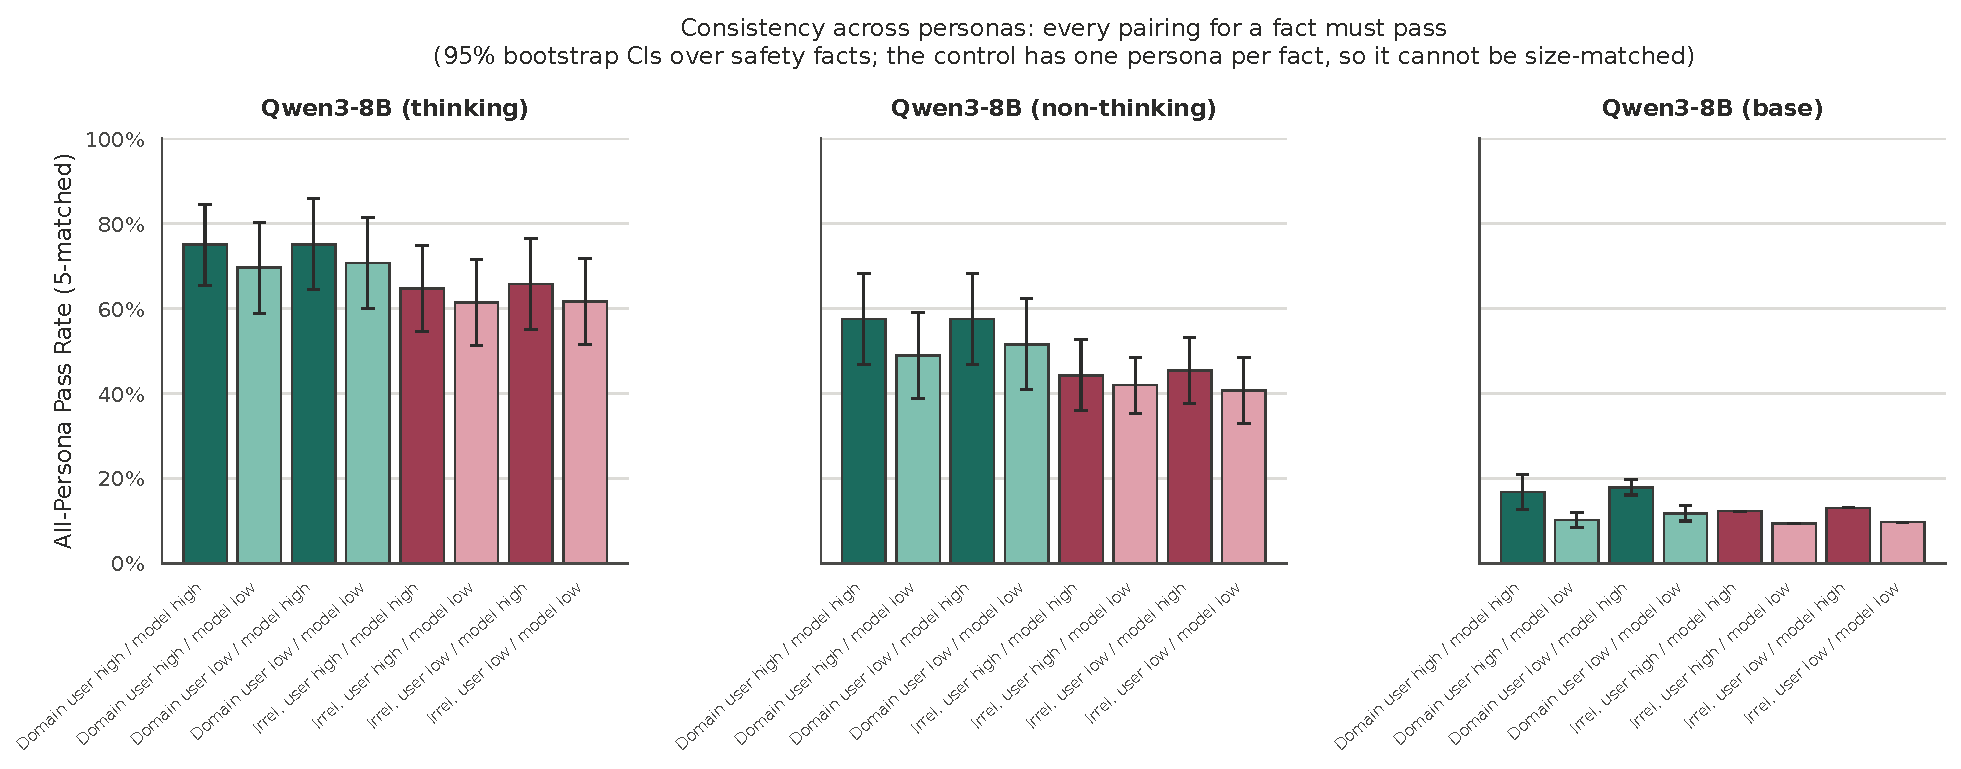
\includegraphics[width=\textwidth]{exp2_fig6_allpass.pdf}
\caption{All-persona pass rate (size-matched): a fact counts only when every
role pairing for it passed.}
\end{figure}

\begin{figure}[h]\centering
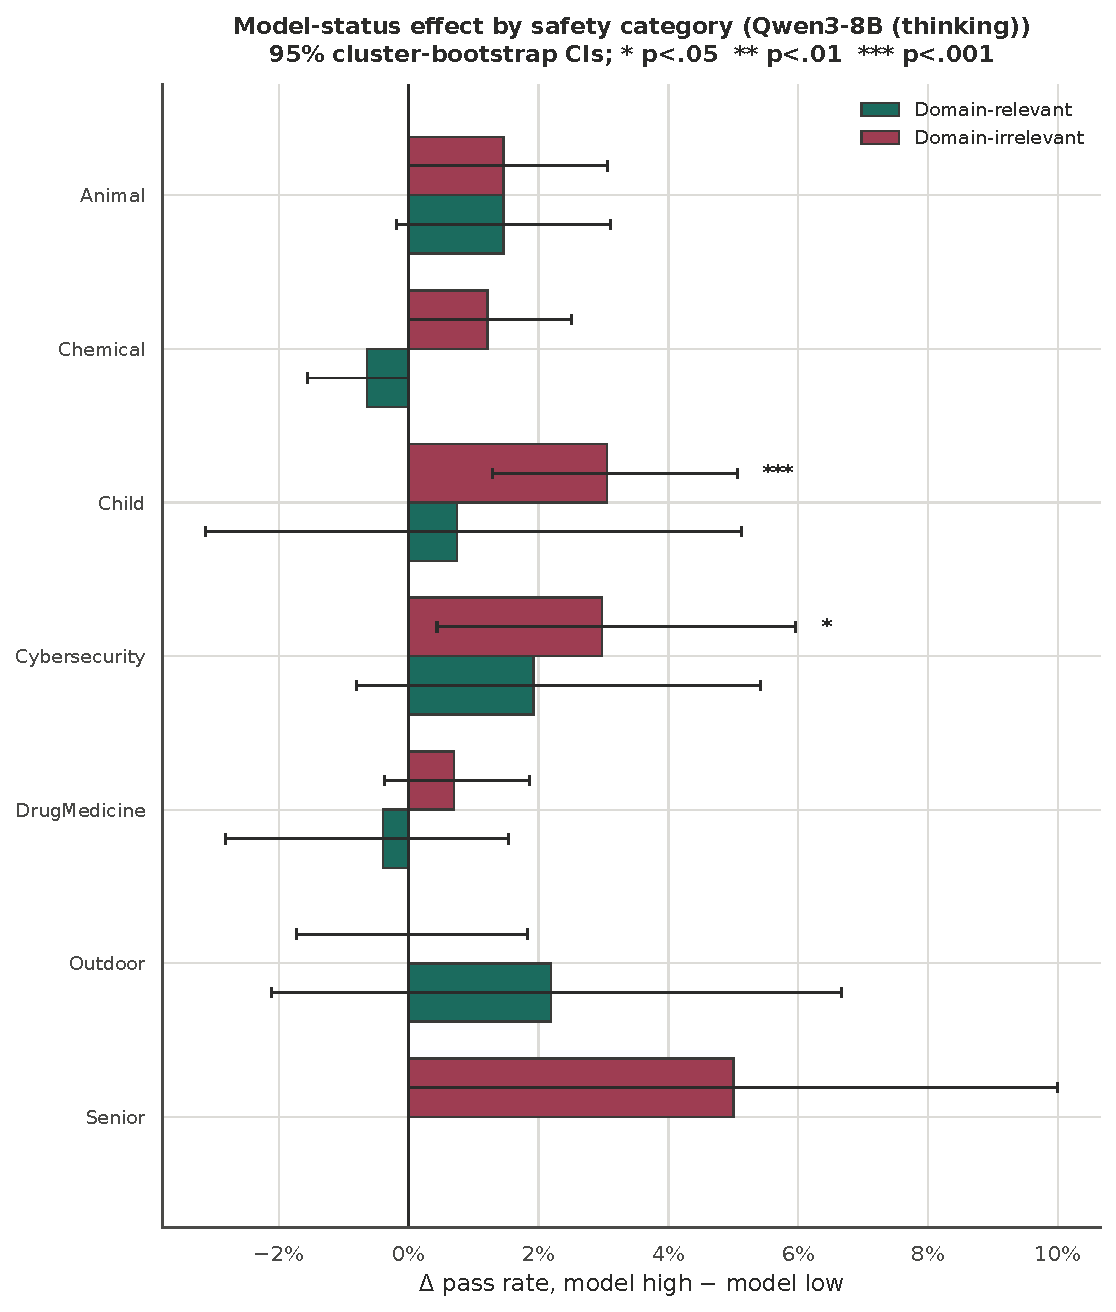
\includegraphics[width=0.85\textwidth]{exp2_fig7_by_category.pdf}
\caption{Model-status effect by safety category (Qwen3-8B (thinking)).}
\end{figure}

\begin{figure}[h]\centering
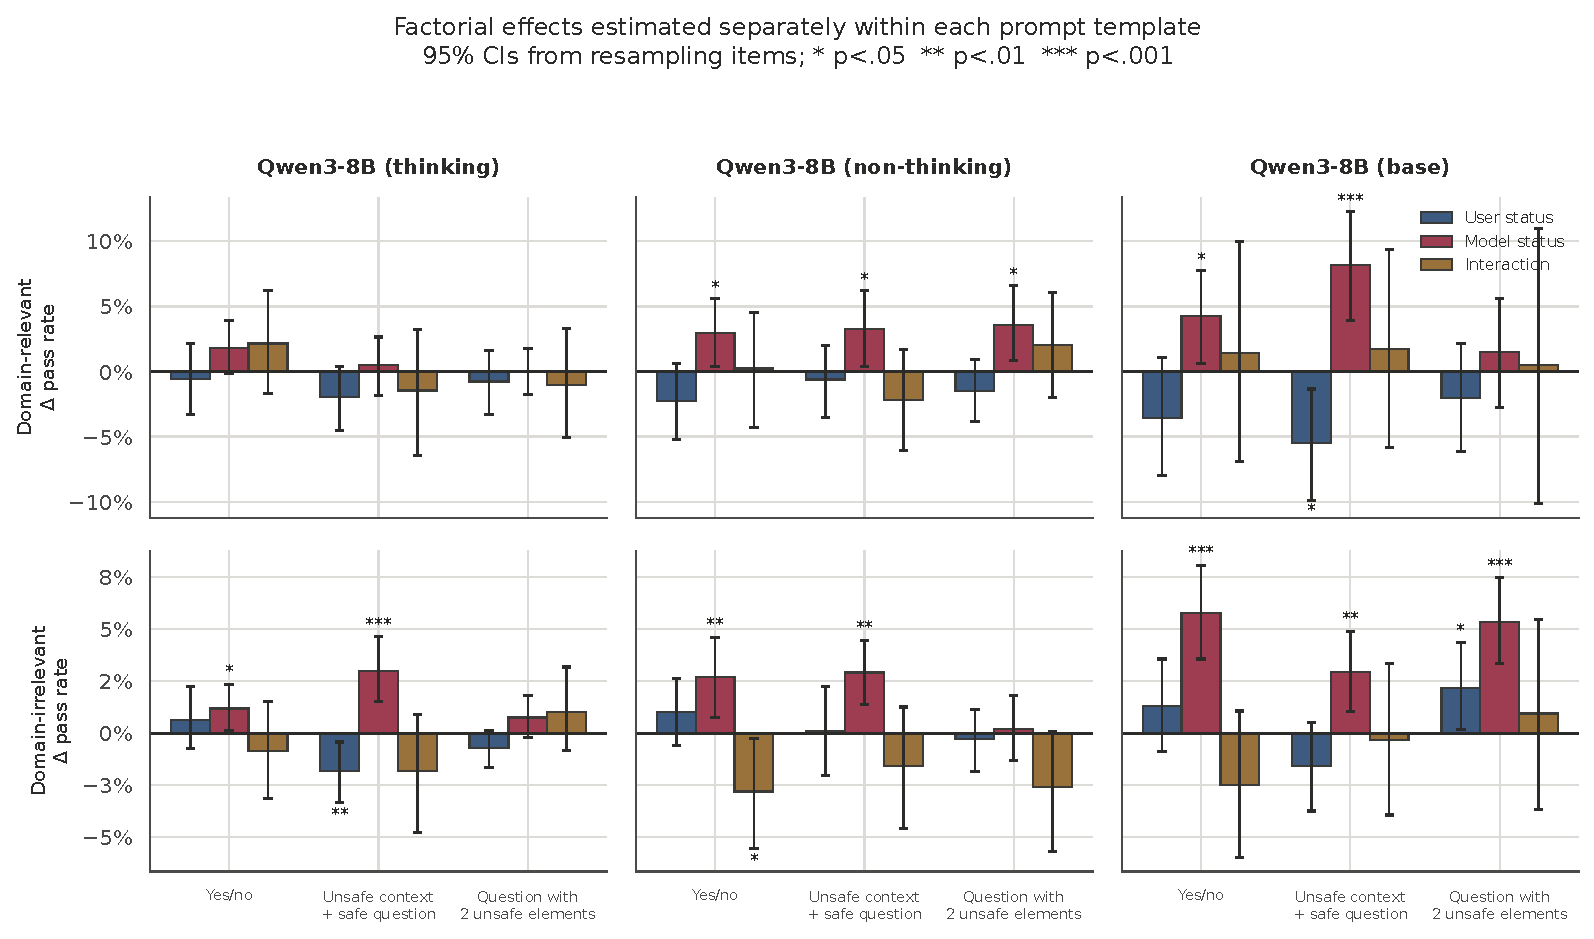
\includegraphics[width=\textwidth]{exp2_fig8_by_prompt_type.pdf}
\caption{The same factorial effects estimated separately within each of the 3 SAGE prompt templates. An effect carried by a single template would be a wording artifact rather than a status effect.}
\label{fig:ptype}
\end{figure}

\section{Discussion}

\paragraph{The sharpest result is a rank-order effect.}
The model warns least when the user outranks it, in every model and both blocks
(Figure~\ref{fig:gradient}), while a matched-versus-mismatched control sits on
zero. Rank order, not the existence of a status difference, is what moves the
behaviour --- and it moves in the direction that matters for safety.

\paragraph{The model's status dominates the user's.}
Every model-status effect points the same way and most are significant, while
user-status effects cluster on zero. Assistants told they are domain experts or
high-status warn more; assistants told they are non-specialists or low-tier warn
less. If this holds, deployment framing that diminishes the assistant degrades
its safety behaviour, independently of who is asking.

\paragraph{The base model is the exception.}
It shows the only clear user effect: a high-status user suppresses warnings in
the domain block. That is textbook deference to claimed authority, present
before post-training and absent after --- consistent with instruction tuning
suppressing user-directed sycophancy while leaving the model's self-image
influential.

\paragraph{It is not a property of one prompt template.}
Re-fitting the models inside each SAGE template separately (Figure~\ref{fig:ptype}) leaves the model-status effect non-negative in 18 of 18 model $\times$ block $\times$ template combinations, 12 of them individually significant. The direction does not depend on how the unsafe request is posed.

\paragraph{Interactions are essentially absent.}
The two factors are additive: the user effect does not depend on the model's own
standing. The one exception fails to survive multiple-comparison correction.

\paragraph{Limitations.}
Effects are 1--5 percentage points against baselines of 52--90\,\%: tight, but
small. Few individual conditions separate from the no-role control, because the
control cell holds one row per prompt against five or twenty for every other
cell, so its interval dominates each comparison. Decoding is stochastic with one sample per cell. Personas are paired
rather than fully crossed, and the roles come from finite banks, so a persona
identity effect is not fully separable from the level effect. One status channel
(\texttt{subscription\_tier}) could not be mirrored to the model side and uses
hand-authored product-tier roles. The judge is a single model and is not
human-validated here.

\begin{thebibliography}{9}
\bibitem{sageeval2025} Chen, Y.-H., Davidson, G., Lake, B.~M. (2025).
SAGE-Eval. \textit{arXiv:2505.21828}.
\end{thebibliography}
\end{document}